\documentclass[border=10pt]{standalone}
\usepackage{pgfplots}
\usepgfplotslibrary{colormaps}
\pgfplotsset{compat=1.18, trig format plots=deg}
\begin{document}
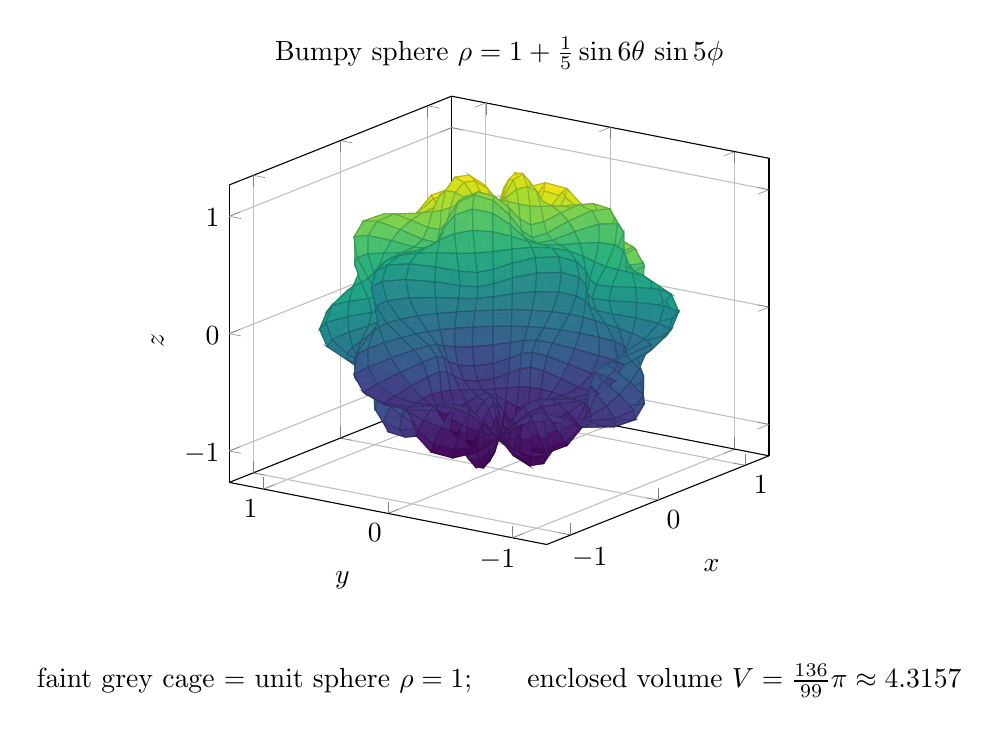
\begin{tikzpicture}
\begin{axis}[domain=0:360, y domain=0:180, samples=49, samples y=25,
             view={-55}{20}, colormap/viridis high res, grid,
             xlabel={$x$}, ylabel={$y$}, zlabel={$z$}, enlargelimits=0.05,
             title={Bumpy sphere $\rho=1+\frac{1}{5}\sin 6\theta\,\sin 5\phi$}]
  \addplot3[fill=black!8, draw=black!45, line width=0.25pt, opacity=0.55,
            samples=25, samples y=17, shader=faceted, faceted color=black!45]
    ({sin(y)*cos(x)}, {sin(y)*sin(x)}, {cos(y)});
  \addplot3[surf, shader=faceted, opacity=0.92]
    ({(1+0.2*sin(6*x)*sin(5*y))*sin(y)*cos(x)},
     {(1+0.2*sin(6*x)*sin(5*y))*sin(y)*sin(x)},
     {(1+0.2*sin(6*x)*sin(5*y))*cos(y)});
\end{axis}
\node[anchor=north, align=center, yshift=-1.4cm] at (current axis.south)
  {faint grey cage = unit sphere $\rho=1$;\qquad enclosed volume $V=\frac{136}{99}\pi\approx 4.3157$};
\end{tikzpicture}
\end{document}
